
\begin{frame}[fragile]{PETSc Application Integration}

\begin{block}{Sparse Matrices}
\begin{itemize}
  \item \textbf{The} important data type when solving PDEs
  \item Two main phases: 
    \begin{itemize}
     \item Filling with entries (assembly)
     \item Application of its action (e.g.~SpMV)
    \end{itemize}
\end{itemize}
\end{block}
\begin{center}
%\includegraphics[width=2in]{figures/Mat/serialSparseMatrix_bcsstk32}
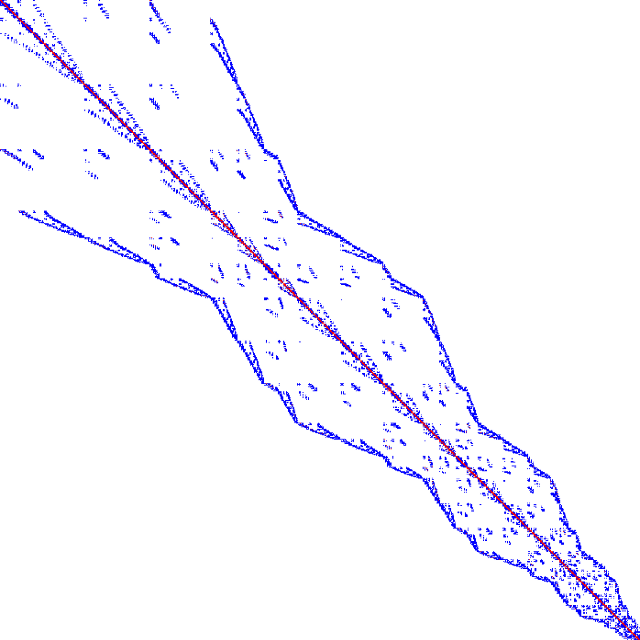
\includegraphics[width=.5\textwidth]{figures/EllipRCMSquare}
\end{center}
\end{frame}



\begin{frame}[fragile]{Matrix Memory Preallocation}
 \begin{block}{PETSc sparse matrices are dynamic data structures}
  \begin{itemize} \vspace*{-0.2cm}
    \item can add additional nonzeros freely
  \end{itemize}
 \end{block}  \vspace*{-0.2cm}

 %\pause
 \begin{block}{Dynamically adding many nonzeros}
  \begin{itemize} \vspace*{-0.2cm}
    \item requires additional memory allocations
    \item requires copies
    \item can kill performance
  \end{itemize}
 \end{block} \vspace*{-0.2cm}

 %\pause
 \begin{block}{Memory preallocation provides}
  \begin{itemize} \vspace*{-0.2cm}
    \item the freedom of dynamic data structures
    \item good performance
  \end{itemize}
 \end{block} \vspace*{-0.2cm}

 %\pause
 \begin{block}{Easiest solution is to replicate the assembly code}
  \begin{itemize} \vspace*{-0.2cm}
    \item Remove computation, but preserve the indexing code
    \item Store set of columns for each row
  \end{itemize}
 \end{block} \vspace*{-0.2cm}

 %\pause
 \begin{block}{Call preallocation routines for all datatypes}
  \begin{itemize} \vspace*{-0.2cm}
    \item \lstinline|MatSeqAIJSetPreallocation()|
    \item \lstinline|MatMPIBAIJSetPreallocation()|
    \item Only the relevant data will be used
  \end{itemize}
\end{block}
\end{frame}




\begin{frame}[fragile]{PETSc Application Integration}

\begin{block}{Sequential Sparse Matrices}
\lstinline|MatSeqAIJSetPreallocation(Mat A, int nz, int nnz[])|
\hbox{\qquad
\vbox{
\begin{itemize}
  \item[nz:] expected number of nonzeros in any row
  \item[nnz(i):] expected number of nonzeros in row i
\end{itemize}
}
}
\end{block}
\begin{center}
%\includegraphics[width=2in]{figures/Mat/serialSparseMatrix_bcsstk32}
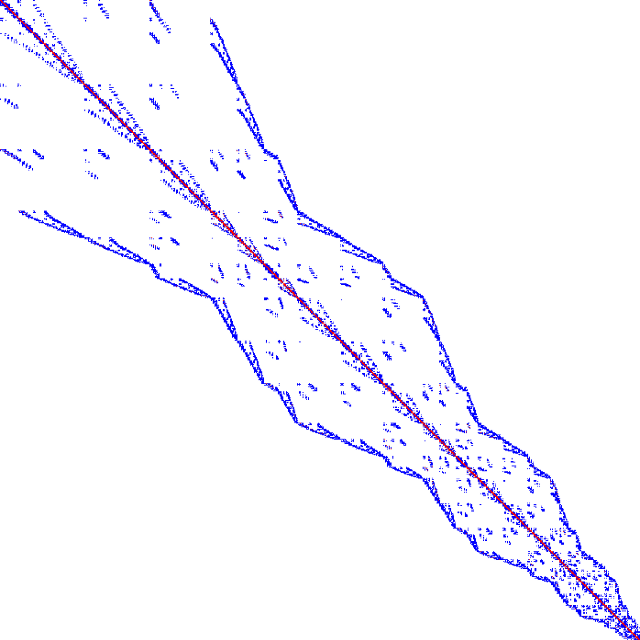
\includegraphics[width=.5\textwidth]{figures/EllipRCMSquare}
\end{center}
\end{frame}

\begin{frame}[fragile]{PETSc Application Integration}

\begin{block}{Parallel Sparse Matrix}
\begin{itemize}
  \item Each process locally owns a submatrix of contiguous global rows
  \item Each submatrix consists of diagonal and off-diagonal parts
\end{itemize}

\begin{center}
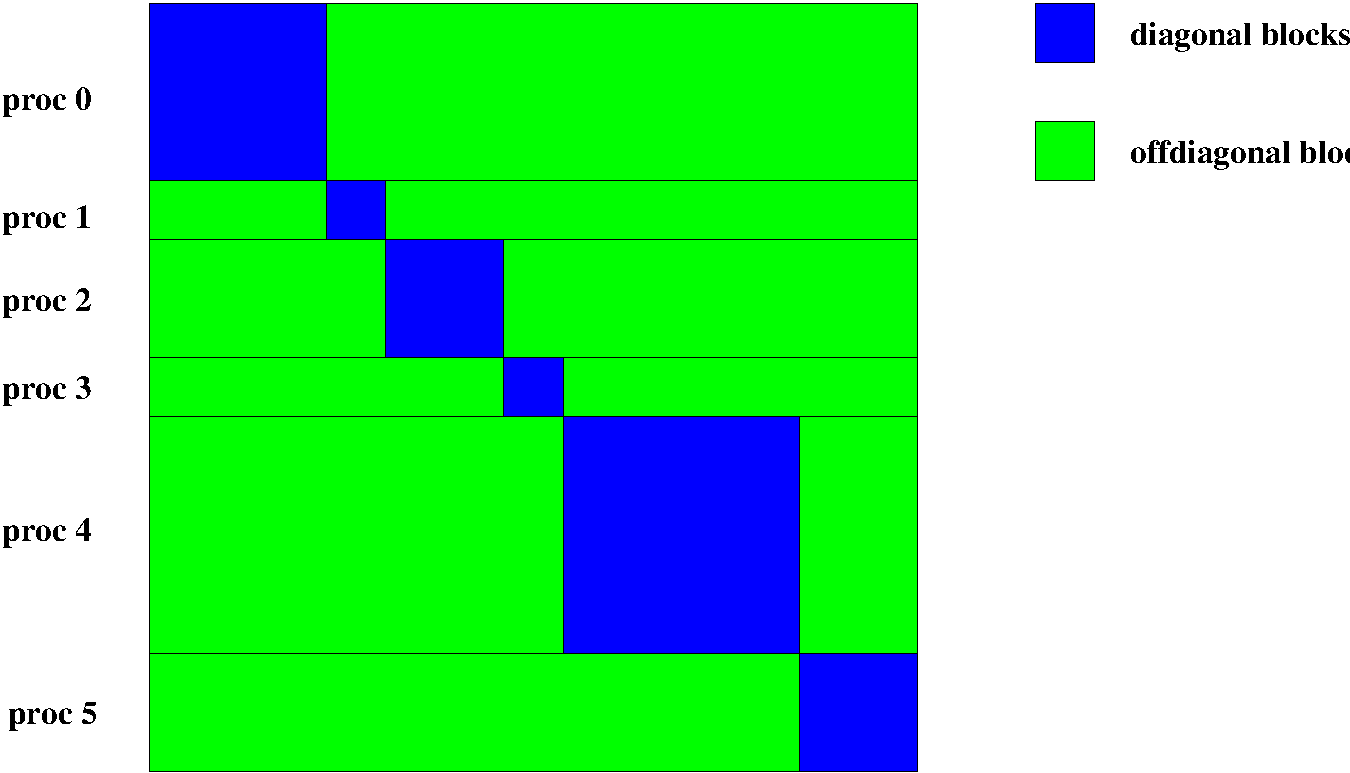
\includegraphics[width=3.in]{figures/Mat/parallelSparseMatrix}
\end{center}

\begin{itemize}
  \item \lstinline|MatGetOwnershipRange(Mat A,int *start,int *end)|
  \begin{itemize}
    \item \lstinline|start|: first locally owned row of global matrix
    \item \lstinline|end-1|: last locally owned row of global matrix
  \end{itemize}
\end{itemize}
\end{block}
\end{frame}


\begin{frame}[fragile]{PETSc Application Integration}

\begin{center}
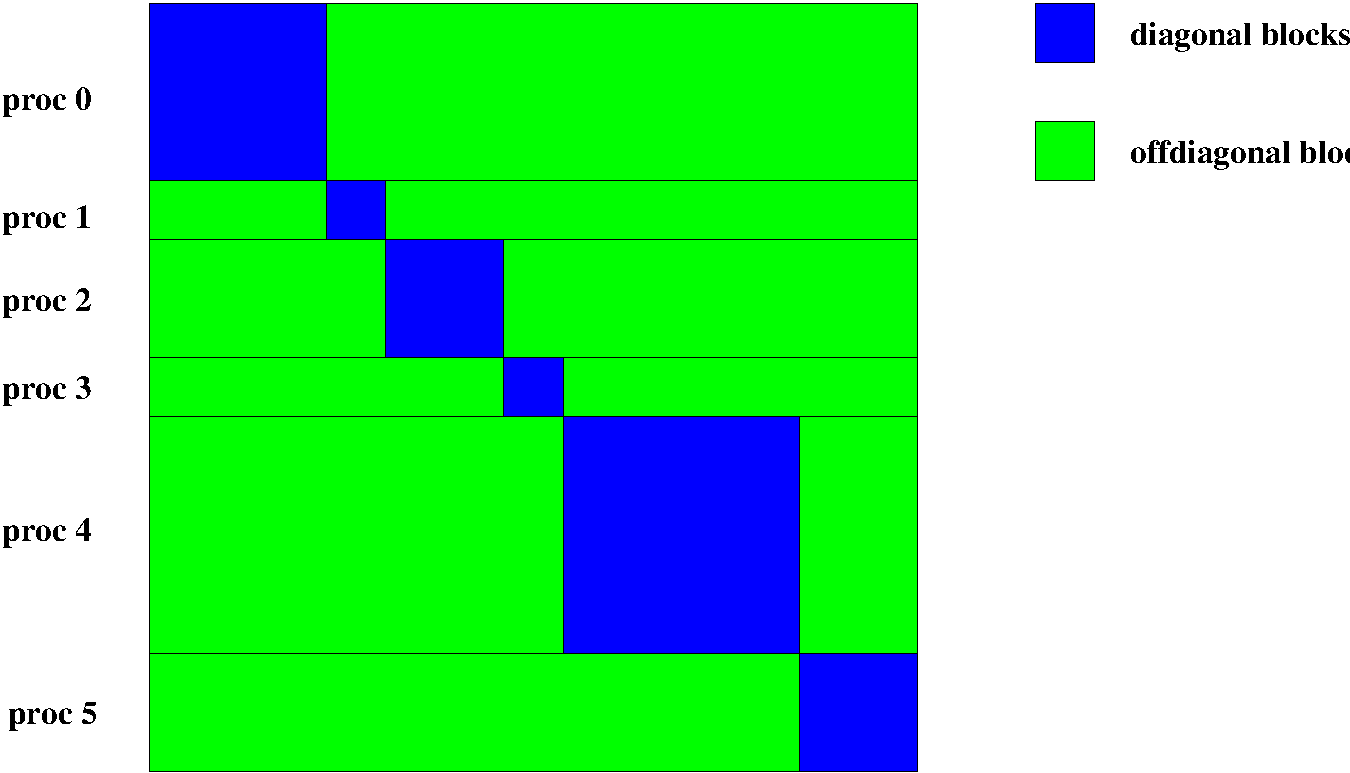
\includegraphics[width=3.in]{figures/Mat/parallelSparseMatrix}
\end{center}

\begin{center}
\begin{tabular}{cc}
\begin{tabular}{c}
\begin{tabular}{|ccc|cc|}
\hline
\multicolumn{3}{|c|}{Proc 2} & \multicolumn{2}{c|}{Proc 3} \\
\hline
25 & 26 & 27 & 28 & 29 \\
20 & 21 & 22 & 23 & 24 \\
15 & 16 & 17 & 18 & 19 \\
\hline
10 & 11 & 12 & 13 & 14 \\
 5 &  6 &  7 &  8 &  9 \\
 0 &  1 &  2 &  3 &  4 \\
\hline
\multicolumn{3}{|c|}{Proc 0} & \multicolumn{2}{c|}{Proc 1} \\
\hline
\end{tabular} \\
Natural numbering
\end{tabular}
& 
\begin{tabular}{c}
\begin{tabular}{|ccc|cc|}
\hline
\multicolumn{3}{|c|}{Proc 2} & \multicolumn{2}{c|}{Proc 3} \\
\hline
21 & 22 & 23 & 28 & 29 \\
18 & 19 & 20 & 26 & 27 \\
15 & 16 & 17 & 24 & 25 \\
\hline
 6 &  7 &  8 & 13 & 14 \\
 3 &  4 &  5 & 11 & 12 \\
 0 &  1 &  2 &  9 & 10 \\
\hline
\multicolumn{3}{|c|}{Proc 0} & \multicolumn{2}{c|}{Proc 1} \\
\hline
\end{tabular}\\
PETSc numbering
\end{tabular}
\end{tabular}
\end{center}

\end{frame}








\begin{frame}[fragile]{PETSc Application Integration}

\begin{block}{Parallel Sparse Matrix}
\vspace{0.5cm}
\hbox{ \quad \vbox{
\begin{lstlisting}
 MatMPIAIJSetPreallocation(Mat A, int dnz, int dnnz[],
                                  int onz, int onnz[]
\end{lstlisting}

\begin{itemize}
  \item[dnz:] expected number of nonzeros in any row in the diagonal block
  \item[dnnz(i):] expected number of nonzeros in row i in the diagonal block
  \item[onz:] expected number of nonzeros in any row in the offdiagonal portion
  \item[onnz(i):] expected number of nonzeros in row i in the offdiagonal portion
\end{itemize}
}}
\end{block}
\end{frame}

\begin{frame}[fragile]{PETSc Application Integration}

\begin{block}{Verifying Preallocation}
\begin{itemize}
  \item Use runtime options 
    \begin{itemize}
      \item \lstinline|-mat_new_nonzero_location_err| 
      \item \lstinline|-mat_new_nonzero_allocation_err|
    \end{itemize}
    
  \item Use runtime option
    \begin{itemize} \item \lstinline|-info| \end{itemize}
  \item Output: \\
\end{itemize}

\end{block}
\begin{lstlisting}[basicstyle=\scriptsize]
[proc #] Matrix size: %d X %d; storage space: %d unneeded, %d used
[proc #] Number of mallocs during MatSetValues( )  is %d
\end{lstlisting}

\begin{center}
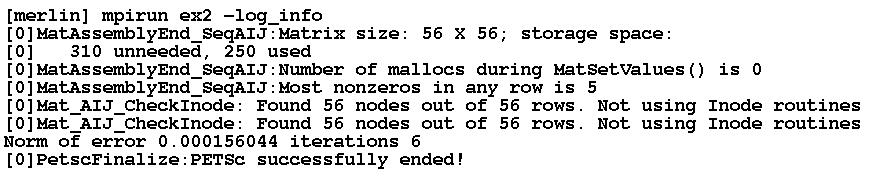
\includegraphics[width=4.in]{figures/logInfoOutput}
\end{center}
\end{frame}

\begin{frame}[fragile]{Block and Symmetric Formats}
  \begin{block}{BAIJ}
    \begin{itemize}
    \item Like AIJ, but uses static block size
    \item Preallocation is like AIJ, but just one index per block
    \end{itemize}
  \end{block}
  
  %\pause
  \begin{block}{SBAIJ}
    \begin{itemize}
    \item Only stores upper triangular part
    \item Preallocation needs number of nonzeros in upper triangular \\
      parts of on- and off-diagonal blocks
    \end{itemize}
  \end{block}
    
  %\pause
  \begin{block}{MatSetValuesBlocked()}
    \begin{itemize}
    \item Better performance with blocked formats
    \item Also works with scalar formats, if \lstinline|MatSetBlockSize()| was called
    \item Variants \lstinline|MatSetValuesBlockedLocal()|, \lstinline|MatSetValuesBlockedStencil()|
    \item Change matrix format at runtime, don't need to touch assembly code
    \end{itemize}
  \end{block}
\end{frame}
